\documentclass{article}
\usepackage[utf8]{inputenc}
\usepackage{vmargin}


\usepackage{amsmath} 
\usepackage{graphicx}
\usepackage{graphics}
\usepackage{float}
\usepackage{blindtext}
\usepackage{listings}
\usepackage{xcolor}
\usepackage[spanish]{babel}
\usepackage{subfig}

\graphicspath{ {images/} }
\title{Operador Logarítmico}
\date{}
\setpapersize{A4}
\setmargins{2.5cm}       % margen izquierdo
{1.5cm}                        % margen superior
{16.5cm}                      % anchura del texto
{23.42cm}                    % altura del texto
{10pt}                           % altura de los encabezados
{1cm}                           % espacio entre el texto y los encabezados
{0pt}                             % altura del pie de página
{2cm}                           % espacio entre el texto y el pie de página

\begin{document}

%-------COLORES PARA CODIGO ------------------------
\lstdefinestyle{customc}{
  belowcaptionskip=1\baselineskip,
  breaklines=true,
  frame=L,
  xleftmargin=\parindent,
  language=JavaScript,
   basicstyle=\footnotesize\ttfamily,
  showstringspaces=false,
  basicstyle=\footnotesize\ttfamily,
  keywordstyle=\bfseries\color{green!40!black},
  commentstyle=\itshape\color{purple!40!black},
  identifierstyle=\color{blue},
  stringstyle=\color{orange},
  frame=single,	  
  numbers=left,
   numberstyle=\footnotesize,
}

\lstdefinestyle{customasm}{
  belowcaptionskip=1\baselineskip,
  frame=L,
  xleftmargin=\parindent,
  language=JavaScript,
  basicstyle=\footnotesize\ttfamily,
  commentstyle=\itshape\color{purple!40!black},
}

\lstset{escapechar=@,style=customc}

%---------------------------------------------

\thispagestyle{empty}

\vfill
 \begin{center}
    \begin{figure}[h]
    \centering
    \includegraphics[width=12cm]{unsa}\\
    
    \end{figure}
 	 
     \vspace*{1.5cm}
    {\large\bfseries FACULTAD DE PRODUCCIÓN Y SERVICIOS} \\
    {\large\bfseries ESCUELA PROFESIONAL DE CIENCIA DE LA COMPUTACIÓN}  \\    
    \vspace*{1.5cm}
    
 	\rule[0.5ex]{\linewidth}{2pt}\vspace*{-\baselineskip}\vspace*		{3.2pt}
	\rule[0.5ex]{\linewidth}{1pt}\\[\baselineskip]
 	{\huge Física Computacional} \\[4mm]
    \rule[0.5ex]{\linewidth}{1pt}\vspace*{-							\baselineskip}\vspace{3.2pt}
	\rule[0.5ex]{\linewidth}{2pt}\\
 	\vspace*{1cm}

    \begin{large} \bfseries
    Tarea aceleración constante \\
    
    \vspace{5mm}
    Eduardo Antonio Sánchez Hincho \\

    \vspace{5mm}
    Docente:\\
    Edwin Agapito Llamoca Requena
    \end{large}
    \vspace*{0.4in}
    
    \noindent \\
    
    \vfill
    \large\bfseries{ AREQUIPA\\2020}
\end{center}
\newpage

\section{Movimiento en una dimensión. Caída libre}
\subsection{}
\begin{itemize}
    \item A
\begin{lstlisting}[language=Python,caption=Ejercicio 1]
h=0.01
x=-10
vx=-20
ax=-10
pt = np.arange(0,10,h)
px=[]
pv=[]
pa=[]
for t in pt:
    x=x+vx*h
    vx=vx+ax*h
    px.append(x)
    pv.append(vx)
    pa.append(ax)
\end{lstlisting}
\begin{figure}[H]
    \centering
    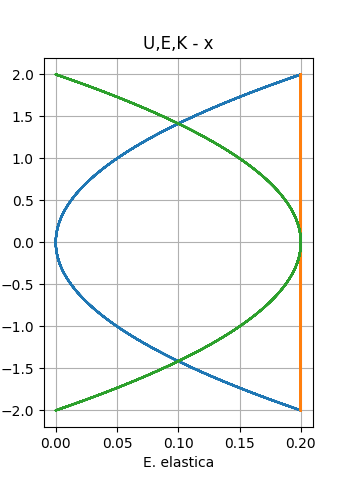
\includegraphics[width=1.21\textwidth]{Figure_2.png}
    \caption{Resultado}
\end{figure}

    \item B
\begin{lstlisting}[language=Python,caption=Ejercicio 2]
h=0.01
x=-10
vx=0
ax=0
pt = np.arange(0,10,h)
px=[]
pv=[]
pa=[]
for t in pt:
    x=x+vx*h
    vx=vx+ax*h
    px.append(x)
    pv.append(vx)
    pa.append(ax)
\end{lstlisting}
    \begin{figure}[H]
    \centering
    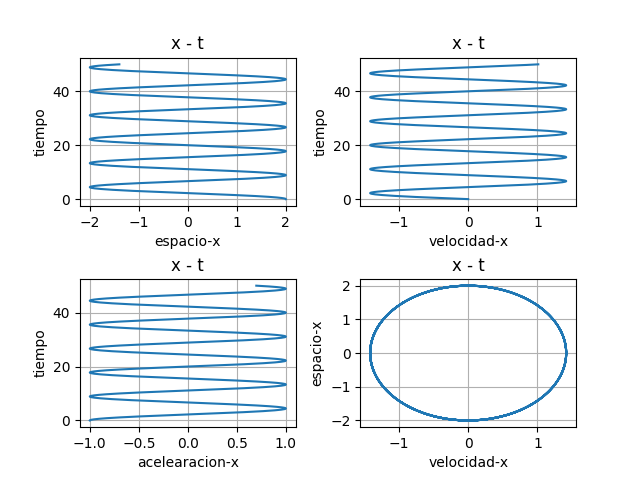
\includegraphics[width=1.21\textwidth]{Figure_1.png}
    \caption{Resultado}
\end{figure}

    \item C
\begin{lstlisting}[language=Python,caption=Ejercicio 3]
h=0.01
x=10
vx=0
ax=0
pt = np.arange(0,10,h)
px=[]
pv=[]
pa=[]
for t in pt:
    x=x+vx*h
    vx=vx+ax*h
    px.append(x)
    pv.append(vx)
    pa.append(ax)
\end{lstlisting}
\begin{figure}[H]
    \centering
    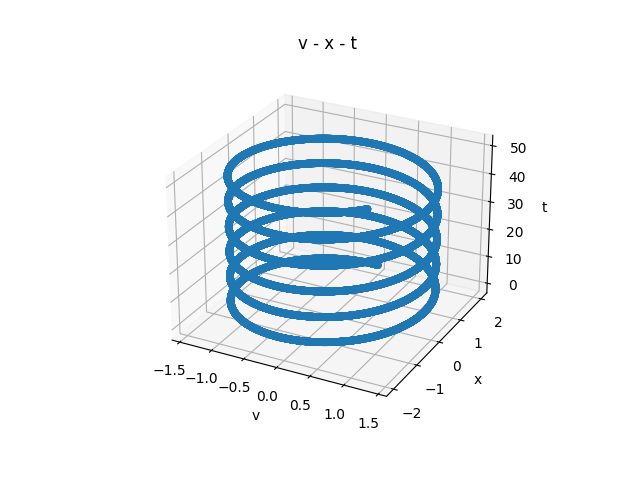
\includegraphics[width=1.21\textwidth]{Figure_3.png}
    \caption{Resultado}
\end{figure}

\end{itemize}

%-----------------------################

\subsection{}
\begin{itemize}
    \item A
\begin{lstlisting}[language=Python,caption=Ejercicio 2.1]
import matplotlib.pyplot as plt
import numpy as np
h=0.05
x=-50
vx=30
ax=10
pt = np.arange(20,0,-h)
px=[]
pv=[]
pa=[]
for t in pt:
    x=x-vx*h
    vx=vx-ax*h
    px.append(x)
    pv.append(vx)
    pa.append(ax)
\end{lstlisting}
\begin{figure}[H]
    \centering
    \includegraphics[width=1.21\textwidth]{Figure_4.png}
    \caption{Resultado}
\end{figure}

    \item B
\begin{lstlisting}[language=Python,caption=Ejercicio 2.1]
import matplotlib.pyplot as plt
import numpy as np
h=0.05
x=-50
vx=0
ax=10
pt = np.arange(20,0,-h)
px=[]
pv=[]
pa=[]
for t in pt:
    x=x-vx*h
    vx=vx-ax*h
    px.append(x)
    pv.append(vx)
    pa.append(ax)
\end{lstlisting}
\begin{figure}[H]
    \centering
    \includegraphics[width=1.21\textwidth]{Figure_5.png}
    \caption{Resultado}
\end{figure}

    \item C
\begin{lstlisting}[language=Python,caption=Ejercicio 2.3]
import matplotlib.pyplot as plt
import numpy as np
h=0.05
x=50
vx=-30
ax=10
pt = np.arange(20,0,-h)
px=[]
pv=[]
pa=[]
for t in pt:
    x=x-vx*h
    vx=vx-ax*h
    px.append(x)
    pv.append(vx)
    pa.append(ax)
\end{lstlisting}
\begin{figure}[H]
    \centering
    \includegraphics[width=1.21\textwidth]{Figure_6.png}
    \caption{Resultado}
\end{figure}

\end{itemize}


%-----------------------################

\subsection{}
\begin{itemize}
    \item A
\begin{lstlisting}[language=Python,caption=Ejercicio 2.2]
import matplotlib.pyplot as plt
import numpy as np
from mpl_toolkits.mplot3d import Axes3D
h=0.01
x=0
vx=15
ax=10
pt = np.arange(0,14,h)
px=[]
pv=[]
pa=[]
for t in pt:
    x=x+vx*h
    vx=vx+ax*h
    px.append(x)
    pv.append(vx)
    pa.append(ax)
    
ax=plt.axes(projection='3d')
ax.set_xlabel('Velocidad')
ax.set_ylabel('Espacio')
ax.set_zlabel('Tiempo')
ax.scatter3D(pv,px,pt,c=pt)
plt.show()
\end{lstlisting}
\begin{figure}[H]
    \centering
    \includegraphics[width=1.21\textwidth]{Figure_7.png}
    \caption{Resultado}
\end{figure}

Para los siguientes ejercicios, los datos son los mismos, solo se varía cosas pequeñas
    \item B

\begin{figure}[H]
    \centering
    \includegraphics[width=1.21\textwidth]{Figure_8.png}
    \caption{Resultado}
\end{figure}

    \item C
\begin{figure}[H]
    \centering
    \includegraphics[width=1.21\textwidth]{Figure_7.png}
    \caption{Resultado}
\end{figure}

\end{itemize}

\section{Movimiento en 2D y 3D con aceleración constante en la dirección Y}
\subsection{}
\begin{lstlisting}[language=Python,caption=Desafío 1.1]
import matplotlib.pyplot as plt
import numpy as np
from mpl_toolkits.mplot3d import Axes3D

h = 0.01
pos = [[0],[0],[0]]
velocidad = [[2],[3],[0]]
a = [0,-10,0]

while True:
    pos[0].append(pos[0][-1] + velocidad[0][-1]*h)
    pos[1].append(pos[1][-1] + velocidad[1][-1]*h)
    pos[2].append(pos[2][-1] + velocidad[2][-1]*h)

    velocidad[0].append(velocidad[0][-1] + a[0]*h)
    velocidad[1].append(velocidad[1][-1] + a[1]*h)
    velocidad[2].append(velocidad[2][-1] + a[2]*h)

    if(pos[1][-1] < 0):
        break
\end{lstlisting}
\begin{figure}[H]
    \centering
    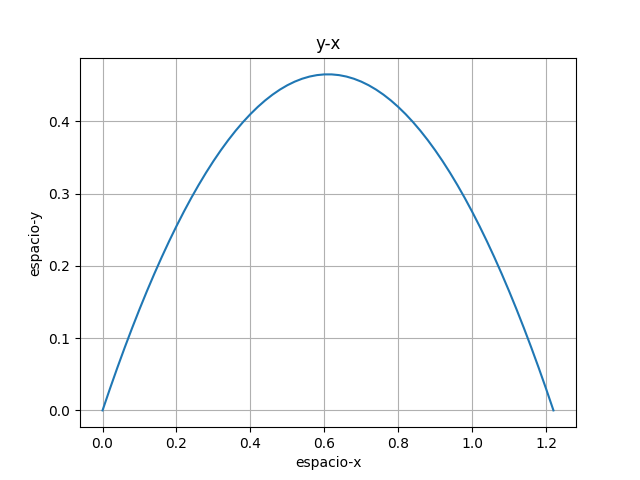
\includegraphics[width=1.21\textwidth]{2_1.png}
    \caption{Resultado}
\end{figure}

\subsection{}
\begin{lstlisting}[language=Python,caption=Desafío 1.1]
h = 0.01
pos = [[-3],[0],[4]]
velocidad = [[2],[3],[4]]
a = [0,-10,0]

while True:
    pos[0].append(pos[0][-1] + velocidad[0][-1]*h)
    pos[1].append(pos[1][-1] + velocidad[1][-1]*h)
    pos[2].append(pos[2][-1] + velocidad[2][-1]*h)

    velocidad[0].append(velocidad[0][-1] + a[0]*h)
    velocidad[1].append(velocidad[1][-1] + a[1]*h)
    velocidad[2].append(velocidad[2][-1] + a[2]*h)

    if(pos[1][-1] < 0):
        break
\end{lstlisting}
\begin{figure}[H]
    \centering
    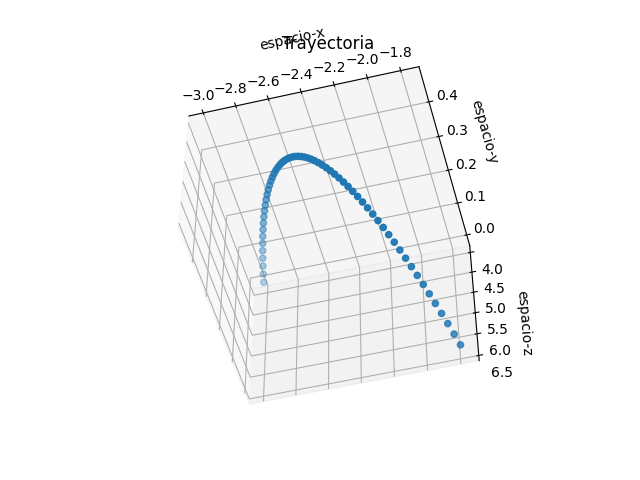
\includegraphics[width=1.21\textwidth]{2_2.png}
    \caption{Resultado}
\end{figure}

\subsection{}
\begin{lstlisting}[language=Python,caption=Desafío 1.1]
h = 0.01
t = 0
pos = [[0],[3],[0]]
velocidad = [[2],[3],[5]]
a = [0,-10,0]
aux = []

while True:
    if velocidad[1][-1] >= 0:
        t += h
        aux = [pos[0][-1],pos[1][-1],pos[2][-1]]

    pos[0].append(pos[0][-1] + velocidad[0][-1]*h)
    pos[1].append(pos[1][-1] + velocidad[1][-1]*h)
    pos[2].append(pos[2][-1] + velocidad[2][-1]*h)

    velocidad[0].append(velocidad[0][-1] + a[0]*h)
    velocidad[1].append(velocidad[1][-1] + a[1]*h)
    velocidad[2].append(velocidad[2][-1] + a[2]*h)

    if(pos[1][-1] < 0):
        break
aux = [round(aux[0],2),round(aux[1],2),round(aux[2],2)]

print(f"Tiempo en que la pelota llega a una altura máxima: {round(t,2)}segundos")
print(f"Coordenadas de mi altua máxima: {aux}")
print(f"El alcance vectorial es: {[round(pos[0][-1]-pos[0][0],2),round(pos[1][-1]-pos[1][0],2),round(pos[2][-1]-pos[2][0],2)]}")

\end{lstlisting}
\begin{figure}[H]
    \centering
    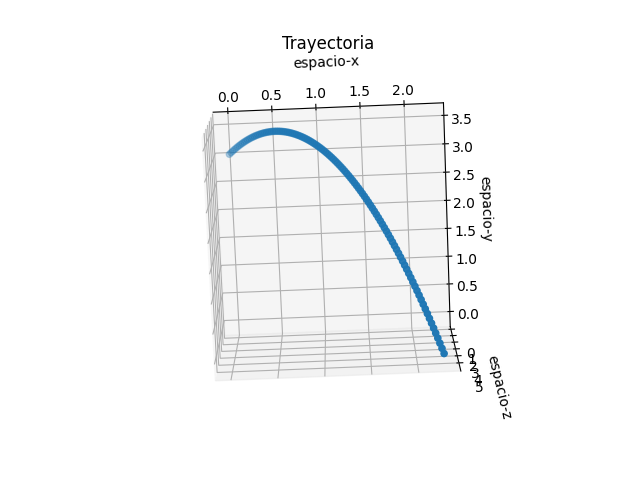
\includegraphics[width=1.21\textwidth]{2_3.png}
    \caption{Resultado}
\end{figure}
\begin{figure}[H]
    \centering
    \includegraphics[width=1\textwidth]{2_3_1.png}
    \caption{Resultado}
\end{figure}

\section{Movimiento en 2D y 3D con aceleración constante en dos direcciones}
\subsection{}
\begin{lstlisting}[language=Python,caption=Desafío 1.1]
h = 0.01
t = 0
pos = [[10],[10],[10]]
velocidad = [[0],[0],[4]]
a = [0,-10,0]

while True:
    pos[0].append(pos[0][-1] + velocidad[0][-1]*h)
    pos[1].append(pos[1][-1] + velocidad[1][-1]*h)
    pos[2].append(pos[2][-1] + velocidad[2][-1]*h)

    velocidad[0].append(velocidad[0][-1] + a[0]*h)
    velocidad[1].append(velocidad[1][-1] + a[1]*h)
    velocidad[2].append(velocidad[2][-1] + a[2]*h)

    if(pos[1][-1] < 0):
        break
\end{lstlisting}
\begin{figure}[H]
    \centering
    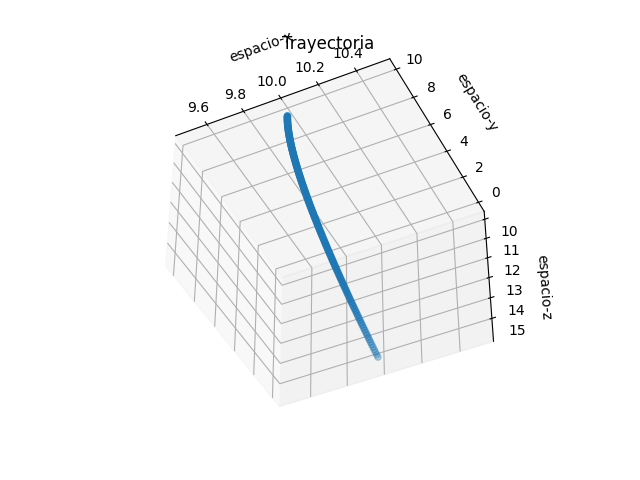
\includegraphics[width=1.21\textwidth]{3_1.png}
    \caption{Resultado}
\end{figure}
\section{}
\begin{figure}[H]
    \centering
    \includegraphics[width=0.5\textwidth]{3_2.jpeg}
    \caption{Resultado}
\end{figure}

\section{Desafío}
\subsection{}
\begin{lstlisting}[language=Python,caption=Desafío 1.1]
h=0.01

pos1 = [[0],[0],[0]]
velocidad1 = [[5],[2],[0]]
a1 = [2,-10,0]

while True:
    pos1[0].append(pos1[0][-1] + velocidad1[0][-1]*h)
    pos1[1].append(pos1[1][-1] + velocidad1[1][-1]*h)
    pos1[2].append(pos1[2][-1] + velocidad1[2][-1]*h)

    velocidad1[0].append(velocidad1[0][-1] + a1[0]*h)
    velocidad1[1].append(velocidad1[1][-1] + a1[1]*h)
    velocidad1[2].append(velocidad1[2][-1] + a1[2]*h)

    if(pos1[1][-1] < 0):
        break
\end{lstlisting}
\begin{figure}[H]
    \centering
    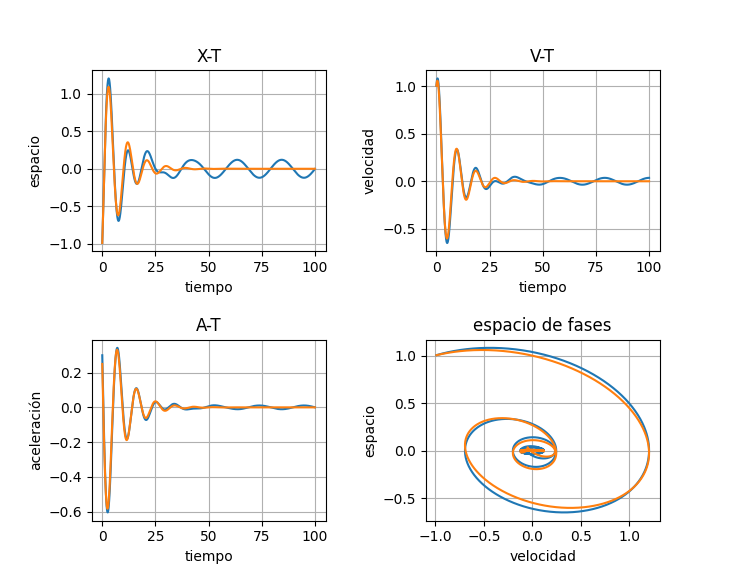
\includegraphics[width=1.21\textwidth]{desa1.png}
    \caption{Resultado}
\end{figure}
\subsection{}
\begin{lstlisting}[language=Python,caption=Desafío 1.2]
h=0.01

pos2 = [[0],[0],[0]]
velocidad2 = [[5],[2],[0]]
a2 = [-1,-10,0]

while True:
    pos2[0].append(pos2[0][-1] + velocidad2[0][-1]*h)
    pos2[1].append(pos2[1][-1] + velocidad2[1][-1]*h)
    pos2[2].append(pos2[2][-1] + velocidad2[2][-1]*h)

    velocidad2[0].append(velocidad2[0][-1] + a2[0]*h)
    velocidad2[1].append(velocidad2[1][-1] + a2[1]*h)
    velocidad2[2].append(velocidad2[2][-1] + a2[2]*h)

    if(pos2[1][-1] < 0):
        break
\end{lstlisting}
\begin{figure}[H]
    \centering
    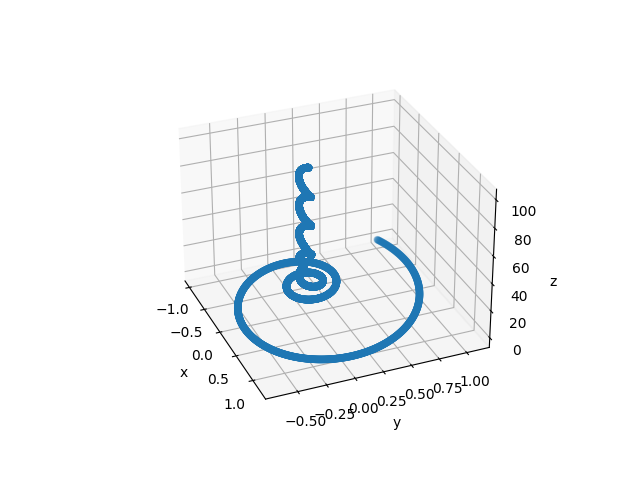
\includegraphics[width=1.21\textwidth]{desa2.png}
    \caption{Resultado}
\end{figure}
\subsection{}
\begin{lstlisting}[language=Python,caption=Desafío 1.3]
h=0.01

pos3 = [[0],[0],[0]]
velocidad3 = [[5],[2],[0]]
a3 = [2,-10,-1]

while True:
    pos3[0].append(pos3[0][-1] + velocidad3[0][-1]*h)
    pos3[1].append(pos3[1][-1] + velocidad3[1][-1]*h)
    pos3[2].append(pos3[2][-1] + velocidad3[2][-1]*h)

    velocidad3[0].append(velocidad3[0][-1] + a3[0]*h)
    velocidad3[1].append(velocidad3[1][-1] + a3[1]*h)
    velocidad3[2].append(velocidad3[2][-1] + a3[2]*h)

    if(pos3[1][-1] < 0):
        break
\end{lstlisting}
\begin{figure}[H]
    \centering
    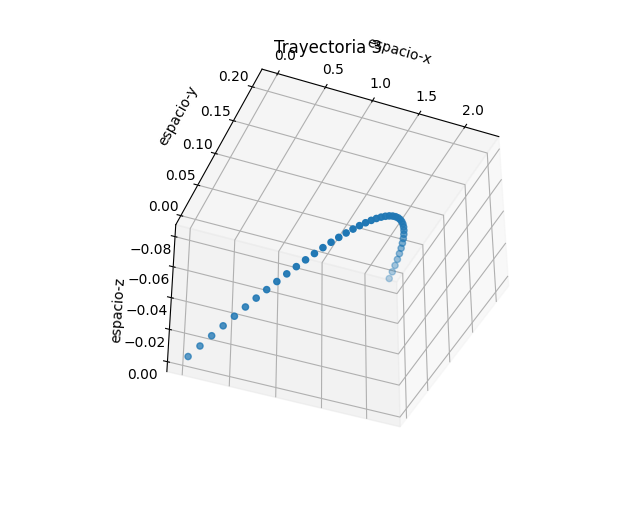
\includegraphics[width=1.21\textwidth]{desa3.png}
    \caption{Resultado}
\end{figure}
\subsection{}

\end{document}


